%%%%%%%%%%%%%%%%%%%%%%%%%%%%%%%%%%%%%%%%%%%%%%%%%%%%%%%%%%%%%%%%%%%%%%%%%%%%%%%
%                         CAPITULO 5
%                  Unidad 5: Encaminadores y Routing
%%%%%%%%%%%%%%%%%%%%%%%%%%%%%%%%%%%%%%%%%%%%%%%%%%%%%%%%%%%%%%%%%%%%%%%%%%%%%%%

\chapter{Encaminadores y Protocolos de Routing}

En los capitulos anteriores hemos visto como los dispositivos se conectan en
redes, como se comunican mediante direcciones IP y como los switches operan
en la capa de enlace. Sin embargo, cuando una red crece y se divide en multiples
subredes, surge un problema fundamental: como hacer que los paquetes de datos
lleguen desde una red a otra, eligiendo el mejor camino posible.

En este capitulo estudiamos el \textbf{encaminamiento} (routing): el proceso de
tomar decisiones sobre por donde enviar los paquetes en una red interconectada.
Veremos los fundamentos teoricos, los algoritmos que permiten calcular caminos
optimos, y los protocolos que permiten a los routers compartir informacion de
rutas automaticamente.


\section{Conceptos fundamentales de encaminamiento}

\begin{definicion}{Encaminamiento y conmutacion}
El \textbf{encaminamiento} (routing) es el proceso de eleccion del camino optimo
que debe seguir un paquete desde su origen hasta su destino a traves de una
red interconectada. Es una decision de control.

La \textbf{conmutacion} (switching) es el acto de retransmitir los datos por uno de
los caminos posibles, una vez tomada la decision. Es una accion de reenvio.
\end{definicion}

El encaminamiento toma la decision sobre el camino a seguir; la conmutacion
ejecuta esa decision reenviando el paquete por la interfaz correspondiente.

\subsection{Tipos de encaminamiento}

Existen varias estrategias para encaminar paquetes:

\begin{itemize}
    \item \textbf{Difusion (Broadcasting)}: envio de informacion a todos los nodos de la
    red. Se implementa mediante \textbf{inundacion} (flooding): cada nodo reenvia el
    paquete a todos sus vecinos excepto al que se lo envio.
    \begin{itemize}
        \item Ventaja: muy robusta, garantiza que se prueban todos los caminos posibles.
        \item Desventaja: mucha sobrecarga, transmisiones y recepciones innecesarias.
    \end{itemize}
    \item \textbf{Camino mas corto (Shortest Path)}: una de las estrategias mas empleadas.
    Se minimiza el numero de saltos entre origen y destino. De manera generica,
    se puede hablar de \textbf{coste} o \textbf{metrica}, estableciendo alguna medida como
    distancia, retardo, ancho de banda, etc.
    \item \textbf{Encaminamiento optimo}: el camino mas corto no siempre ofrece el mejor
    comportamiento (por ejemplo, puede estar congestionado). El encaminamiento
    optimo busca la mejor ruta segun multiples criterios mediante optimizacion
    matematica.
    \item \textbf{Patata caliente (Hot Potato)}: un nodo manda cada paquete por la interfaz
    menos cargada, deshaciendose del mismo lo antes posible. Es una tecnica muy
    simple que no considera la distancia global.
\end{itemize}


\section{Grafos y encaminamiento}

Los \textbf{grafos} son una herramienta matematica que se emplea para formular
problemas de encaminamiento.

\begin{definicion}{Grafo}
Un \textbf{grafo} es una estructura matematica definida como G = (N, d), donde:
\begin{itemize}
    \item \textbf{N} es un conjunto de nodos (vertices).
    \item \textbf{d} es una coleccion de enlaces (edges), donde cada enlace consta de un
    par de nodos de N.
\end{itemize}
\end{definicion}

Al trasladar un grafo a un problema de encaminamiento:
\begin{itemize}
    \item Los \textbf{nodos} N son los encaminadores (routers) de la red.
    \item Los \textbf{enlaces} d se corresponden con los enlaces fisicos entre ellos.
\end{itemize}

\subsection{Tipos de grafos}

\begin{itemize}
    \item \textbf{Grafos dirigidos}: los enlaces son pares ordenados (u,v) donde el
    orden importa. (u,v) $\neq$ (v,u).
    \item \textbf{Grafos no dirigidos}: los enlaces no tienen direccion. (u,v) = (v,u).
\end{itemize}

\subsection{Concatenaciones de enlaces}

\begin{itemize}
    \item \textbf{Paseo (Walk)}: secuencia de nodos (n1, n2, ..., nl) tal que cada pareja
    (ni-1, ni) es un enlace del grafo.
    \item \textbf{Camino (Path)}: es un paseo en el que no hay nodos repetidos.
    \item \textbf{Ciclo o bucle (Cycle)}: camino con mas de un enlace en el que el nodo
    inicial coincide con el final (n1 = nl).
\end{itemize}

\subsection{Grafo conectado}

Se dice que un grafo esta \textbf{conectado} si cualquier par de nodos esta conectado
por un camino. En redes de comunicaciones, esto significa que cualquier router
puede comunicarse con cualquier otro.

\subsection{Representacion de grafos}

Los grafos se pueden representar de dos formas principales:

\begin{table}[htbp]
\centering
\small
\caption{Representacion de grafos}
\begin{tabularx}{\textwidth}{@{}l>{\raggedright\arraybackslash}X>{\raggedright\arraybackslash}X@{}}
\toprule
\textbf{Aspecto} & \textbf{Lista de adyacencia} & \textbf{Matriz de adyacencia} \\
\midrule
Estructura & Array de N listas, una por nodo, con punteros a vecinos & Matriz F de dimension N x N \\
Memoria & Menor memoria, apropiada para grafos dispersos (sparse) & Mayor memoria, N\^{}2 elementos \\
Ventajas & Eficiente en memoria para grafos con pocos enlaces & Busqueda muy rapida, facil asignar costes \\
Desventajas & Busqueda puede ser lenta & Requiere mas memoria, se usa en grafos pequenos \\
Grafos no dirigidos & Numero de punteros = 2|d| & Matriz simetrica: F\^{}T = F \\
Grafos dirigidos & Numero de punteros = |d| & Matriz no simetrica \\
\bottomrule
\end{tabularx}
\end{table}

\subsection{Costes en los enlaces}

En algunas ocasiones se asignan \textbf{costes} c(u,v) a los enlaces, representando
metricas como:
\begin{itemize}
    \item Distancia fisica (kilometros).
    \item Retardo (milisegundos).
    \item Ancho de banda (Mbps).
    \item Congestion actual.
\end{itemize}

El objetivo del encaminamiento es entonces encontrar el camino con menor coste
acumulado.


\section{Algoritmos de camino mas corto}

La idea principal es encontrar el camino con un coste minimo entre una fuente
(S) y un destino (D). Si c(u,v) se mantiene constante para todos los enlaces,
la solucion es la ruta de menor numero de saltos.

\subsection{Algoritmos con una unica fuente}

Encuentran el camino mas corto entre un nodo origen S y el resto de nodos:

\begin{itemize}
    \item \textbf{Dijkstra}: funciona con grafos donde los costes son positivos.
    Es el algoritmo mas utilizado en protocolos como OSPF.
    \item \textbf{Bellman-Ford}: permite costes negativos (si no hay ciclos negativos).
    Es la base del encaminamiento por vectores de distancia (RIP).
\end{itemize}

\subsection{Algoritmos para toda la red}

Encuentran el camino mas corto entre todas las posibles parejas de nodos:

\begin{itemize}
    \item \textbf{Floyd-Warshall}: algoritmo de programacion dinamica.
    \item \textbf{Johnson}: combina Dijkstra y Bellman-Ford para grafos dispersos.
\end{itemize}

\subsection{Arbol de expansion minimo (Minimum Spanning Tree)}

Un \textbf{arbol} es un grafo no dirigido, conectado y sin ciclos. El numero de
enlaces es igual al numero de nodos menos 1: |d| = |N| - 1.

Un \textbf{Spanning Tree} cubre (se expande por) todos los nodos de un grafo. El
\textbf{Minimum Spanning Tree (MST)} es aquel que tiene el menor coste total.

\textbf{Aplicaciones}:
\begin{itemize}
    \item Procesos de difusion (broadcast) de informacion.
    \item Redes de area local: bridges (IEEE 802.1D) emplean el MST para eliminar
    enlaces no necesarios y evitar bucles.
\end{itemize}

\textbf{Algoritmos}: Kruskal y Prim.


\section{Protocolos de encaminamiento}

Los nodos (encaminadores) toman decisiones en base a cierta informacion. Es
necesario disponer de un \textbf{protocolo de senalizacion} que proporcione un metodo
para transportar dicha informacion por la red.

\subsection{Clasificacion de protocolos}

\begin{table}[htbp]
\centering
\small
\caption{Clasificacion de protocolos de encaminamiento}
\begin{tabularx}{\textwidth}{@{}l>{\raggedright\arraybackslash}X@{}}
\toprule
\textbf{Tipo} & \textbf{Descripcion} \\
\midrule
Vector de distancia (DV) & Cada router intercambia periodicamente su tabla con los vecinos. Usa Bellman-Ford. Ejemplo: RIP. \\
Estado de enlace (LS) & Cada router difunde el estado de sus enlaces a toda la red. Usa Dijkstra. Ejemplo: OSPF. \\
\bottomrule
\end{tabularx}
\end{table}

\subsection{Encaminamiento por vector de distancia}

Se basa en el algoritmo de Bellman-Ford. Cada nodo de la red mantiene una tabla
de encaminamiento con una entrada por cada uno del resto de nodos:

\begin{itemize}
    \item \textbf{Distancia}: metrica o coste del camino hacia dicho nodo.
    \item \textbf{Interfaz de salida}: necesaria para alcanzarle.
\end{itemize}

Periodicamente, cada nodo intercambia la informacion de su tabla con sus vecinos.

\textbf{Problemas}:
\begin{itemize}
    \item \textbf{Convergencia lenta}: los cambios en la topologia tardan en propagarse.
    \item \textbf{Propagacion rapida de ``buenas noticias'' y lenta de las ``malas''}:
    cuando un enlace mejora, la noticia se propaga rapido; cuando empeora, tarda.
    \item \textbf{Count-to-infinity}: si un enlace cae, los routers pueden incrementar
    sus metricas hasta el infinito de forma ciclica.
\end{itemize}

\textbf{Soluciones al count-to-infinity}:
\begin{itemize}
    \item \textbf{Limitar el infinito}: en RIP, el limite es 16 saltos (una red a 16
    saltos se considera inalcanzable).
    \item \textbf{Horizonte dividido (Split Horizon)}: un router no anuncia una ruta
    de regreso a la interfaz por la que la aprendio.
    \item \textbf{Horizonte dividido con respuesta envenenada (Poison Reverse)}: si
    se anuncia la ruta de regreso, se hace con distancia infinita.
    \item \textbf{Actualizaciones forzadas (Triggered Updates)}: cuando un router detecta
    un cambio, difunde inmediatamente la informacion sin esperar al temporizador.
\end{itemize}

\subsection{Encaminamiento por estado de enlace}

\textbf{Desventajas}:
\begin{itemize}
    \item Necesidad de informacion global sobre la red.
    \item Envio de un numero mayor de mensajes: sobrecarga.
    \item Un evento de cambio en la topologia debe notificarse a todos los nodos.
\end{itemize}

\textbf{Protocolo OSPF} (Open Shortest Path First):
\begin{itemize}
    \item Definido en el RFC 2328 (version 2).
    \item Es un protocolo Intra-AS (dentro de un Sistema Autonomo).
    \item Utiliza el algoritmo de Dijkstra.
    \item Cada router conoce la topologia completa de la red.
\end{itemize}

\subsection{Encaminamiento jerarquico: Sistemas Autonomos (AS)}

Internet esta organizada en \textbf{Sistemas Autonomos} (AS):

\begin{definicion}{Sistema Autonomo (AS)}
Un \textbf{Sistema Autonomo (AS)} es una coleccion de redes y encaminadores
gestionadas y administradas por una misma autoridad (por ejemplo, un ISP, una
universidad, una empresa).
\end{definicion}

\begin{itemize}
    \item \textbf{Encaminadores internos del AS}: interconectan redes dentro del
    propio AS. Solo conocen en detalle la organizacion local. Utilizan protocolos
    \textbf{IGP} (Interior Gateway Protocol).
    \item \textbf{Encaminadores externos o frontera (border router)}: interconectan
    varios sistemas autonomos. Conocen el camino al resto de AS, pero no en
    detalle. Utilizan protocolos \textbf{EGP} (Exterior Gateway Protocol).
\end{itemize}

\textbf{Protocolos IGP} (dentro de un AS):
\begin{itemize}
    \item \textbf{RIP}: Routing Information Protocol.
    \item \textbf{OSPF}: Open Shortest Path First.
    \item \textbf{IGRP}: Internal Gateway Routing Protocol (de Cisco).
\end{itemize}

\textbf{Protocolos EGP} (entre AS):
\begin{itemize}
    \item \textbf{BGP}: Border Gateway Protocol. Es el protocolo que sostiene Internet,
    permitiendo que los diferentes AS intercambien informacion de rutas.
\end{itemize}


\section{Protocolo RIP (Routing Information Protocol)}

\subsection{Caracteristicas generales}

RIP es un protocolo de encaminamiento interior (IGP) basado en vectores de
distancia (algoritmo Bellman-Ford).

\begin{table}[htbp]
\centering
\small
\caption{Versiones de RIP}
\begin{tabularx}{\textwidth}{@{}l>{\raggedright\arraybackslash}X@{}}
\toprule
\textbf{Version} & \textbf{Caracteristicas} \\
\midrule
RIP v1 (RFC 1058, 1993) & No soporta VLSM/CIDR, envia broadcast \\
RIP v2 (RFC 2453, 1998) & Soporta VLSM/CIDR, envia multicast, incluye mascara \\
RIPng (RFC 2080, 1997) & Version para IPv6, puerto UDP 521, multicast FF02::9 \\
\bottomrule
\end{tabularx}
\end{table}

Los vectores de distancia incluyen:
\begin{itemize}
    \item La lista de destinos (redes) alcanzables por cada router.
    \item La distancia (numero de saltos) a dichos destinos.
\end{itemize}

La metrica de RIP es el \textbf{numero de saltos}. El limite de infinito es 16 saltos.
RIP utiliza los puertos UDP 520 (RIPv2) y 521 (RIPng).

\subsection{Temporizadores de RIP}

RIP utiliza tres temporizadores principales:

\begin{itemize}
    \item \textbf{Temporizador periodico} (25-35 s): intervalo de envio de mensajes
    RESPONSE para anunciar vectores de distancia. El valor oficial es 30 s, pero
    en la practica se usa un valor aleatorio entre 25 y 35 s para evitar
    sincronizacion.
    \item \textbf{Temporizador de expiracion} (180 s): controla el periodo de validez
    de una entrada. Si no se recibe actualizacion durante 180 s (equivalente a
    3 intervalos periodicos), la entrada deja de considerarse valida.
    \item \textbf{Temporizador de ``coleccion de basura''} (120 s): cuando una entrada
    expira, no se elimina inmediatamente. Se sigue anunciando con metrica 16
    (destino inalcanzable) durante 120 s adicionales para notificar a los vecinos.
\end{itemize}

\subsection{Mensajes RIP}

\begin{itemize}
    \item \textbf{REQUEST}: enviados por un router cuando se conecta a la red, o cuando
    caduca una entrada.
    \item \textbf{RESPONSE}: enviados periodicamente con los vectores de distancia, en
    respuesta a una solicitud, o como actualizacion forzada cuando cambia la
    distancia a una red.
\end{itemize}

\subsection{RIPng para IPv6}

RIPng (RIP new generation) es la adaptacion de RIP-2 para IPv6:
\begin{itemize}
    \item Los mensajes se encapsulan en datagramas UDP dirigidos al puerto 521.
    \item Se difunden a la direccion IPv6 multicast FF02::9.
    \item Los vectores de distancia anuncian prefijos de red IPv6 en lugar de
    direcciones IPv4.
    \item No incluye el campo ``Next Hop'' en cada entrada (se usa un mecanismo
    separado).
    \item No utiliza autenticacion propia; delega a los mecanismos de IPv6.
\end{itemize}


\section{Tablas de Encaminamiento}

\subsection{Encaminamiento ``Next-Hop''}

\begin{definicion}
El principio de encaminamiento \textbf{Next-Hop} se basa en la optimizacion: si el camino mas corto entre A y D pasa por B, entonces el camino mas corto de B a D es la misma ruta. Por tanto, solo se necesita conocer el \textbf{siguiente encaminador inmediato} (next hop), no la ruta completa.
\end{definicion}

\begin{figure}[H]
\centering
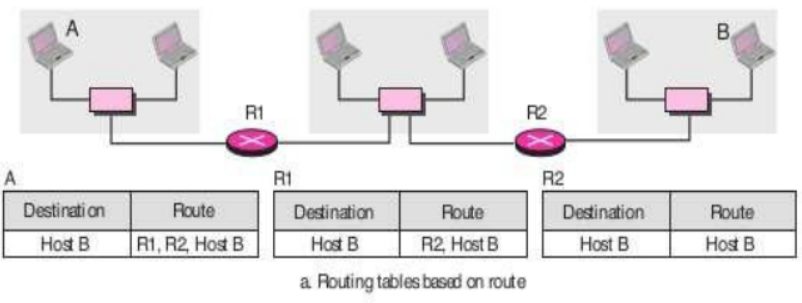
\includegraphics[width=0.8\textwidth]{assets/cap5/5.1.png}
\caption{Principio de encaminamiento next-hop}
\label{fig:next-hop}
\end{figure}

\subsection{Estructura de una tabla de encaminamiento}

Una tabla de encaminamiento contiene las siguientes entradas:

\begin{itemize}
    \item \textbf{Destino}: red o host de destino.
    \item \textbf{Mascara o prefijo de red (CIDR)}: define la porcion de red de la direccion.
    \item \textbf{Siguiente salto (next hop)}: direccion del siguiente router hacia el destino.
    \item \textbf{Coste}: metrica asociada al camino.
\end{itemize}

Tipos de entrada destino:
\begin{itemize}
    \item \textbf{Host especifico}: no viable en Internet por el gran numero de equipos.
    \item \textbf{Red}: con prefijo CIDR, la entrada mas utilizada.
    \item \textbf{Default}: para paquetes sin coincidencia en las demas entradas.
\end{itemize}

\begin{figure}[H]
\centering
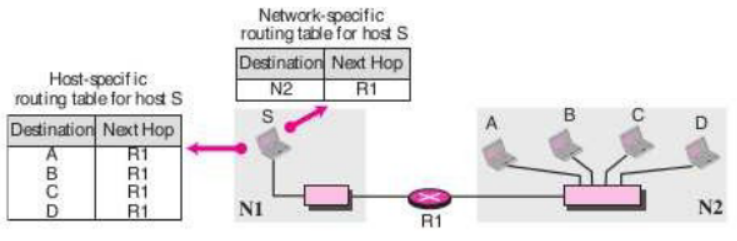
\includegraphics[width=0.8\textwidth]{assets/cap5/5.2.png}
\caption{Ejemplo de tabla de encaminamiento}
\label{fig:tabla-encaminamiento}
\end{figure}

\subsection{Ejemplo practico}

Dada una topologia de red con varios routers:
\begin{enumerate}
    \item Determinar la tabla de encaminamiento del router R1.
    \item Procesar paquetes con destino \texttt{201.4.22.35} y \texttt{18.24.32.78}.
\end{enumerate}

\begin{figure}[H]
\centering
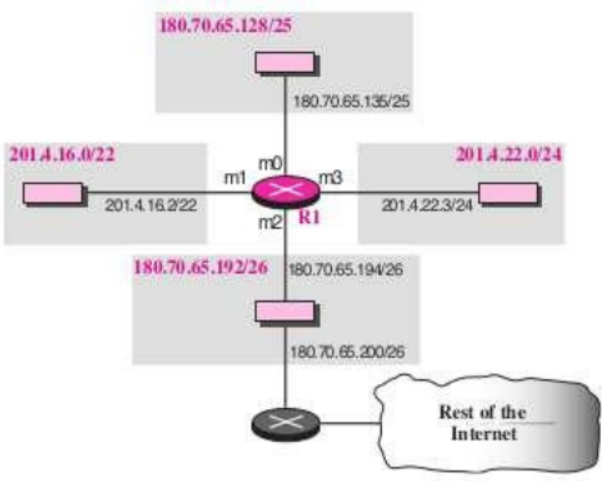
\includegraphics[width=0.8\textwidth]{assets/cap5/5.3.png}
\caption{Topologia de red del ejemplo con routers}
\label{fig:topologia-ejemplo}
\end{figure}

\subsection{Escalabilidad}

El encaminamiento con clase no es viable por el gran numero de redes. Soluciones:
\begin{itemize}
    \item \textbf{CIDR}: agregacion de direcciones y resumen de rutas.
    \item \textbf{Encaminamiento jerarquico}: limita la informacion intercambiada entre dominios.
\end{itemize}

\begin{figure}[H]
\centering
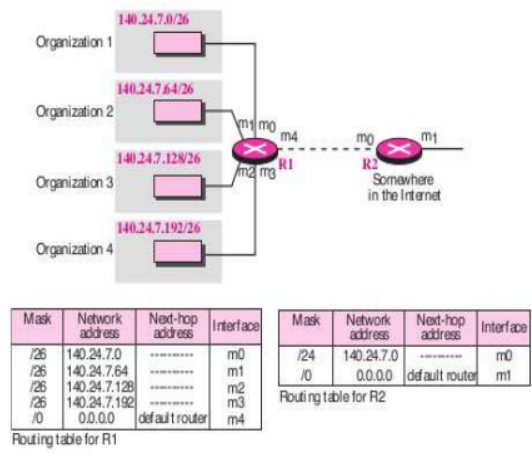
\includegraphics[width=0.8\textwidth]{assets/cap5/5.4.png}
\caption{Agregacion CIDR y jerarquia de encaminamiento}
\label{fig:cidr-jerarquia}
\end{figure}


\section{Tecnicas de Encaminamiento}

\subsection{Encaminamiento local}

No usa topologia global, solo informacion local.

\begin{itemize}
    \item \textbf{Aleatorio}: elige una salida al azar. Simple pero no optimo.
    \item \textbf{Aislado}: usa informacion local (mayor ancho de banda, menor congestion, round-robin).
    \item \textbf{Por inundacion (flooding)}: envia el paquete a todos los vecinos menos al origen.
\end{itemize}

\begin{definicion}
El \textbf{encaminamiento por inundacion (flooding)} es una tecnica en la que cada nodo reenvia el paquete recibido a todos sus vecinos excepto a aquel del que lo recibio. El destinatario puede recibir copias duplicadas, por lo que se usa un identificador unico para descartarlas. Se emplea el campo TTL para evitar bucles infinitos.
\end{definicion}

Ventajas del flooding: robusto, garantiza el camino mas corto, visita todos los nodos. Desventajas: saturacion por duplicados.

\begin{figure}[H]
\centering
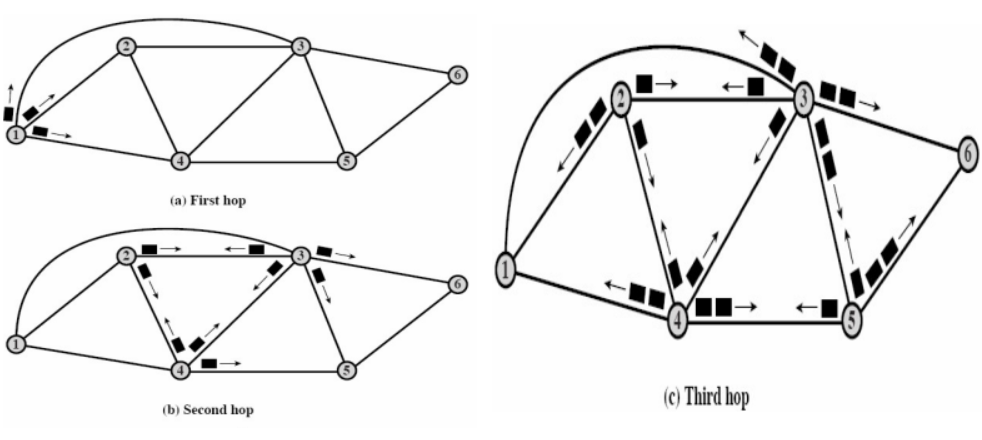
\includegraphics[width=0.8\textwidth]{assets/cap5/5.5.png}
\caption{Ejemplo de inundacion en red con multiples routers}
\label{fig:flooding-ejemplo}
\end{figure}

\subsection{Encaminamiento estatico}

Considera la topologia de la red. Las tablas se construyen \textbf{manualmente} y no se adaptan a cambios en la red.




\section{Vectores de Distancia}

\subsection{Fundamentos}

\begin{definicion}
En el \textbf{encaminamiento por vectores de distancia}, cada encaminador mantiene una entrada por cada destino posible con: destino, siguiente nodo y distancia/metria. El intercambio periodico de estos vectores con los vecinos permite que la red converja a caminos optimos mediante el algoritmo de \textbf{Bellman-Ford}. La metrica tipica es el \textbf{numero de saltos} (hop count).
\end{definicion}

\begin{figure}[H]
\centering
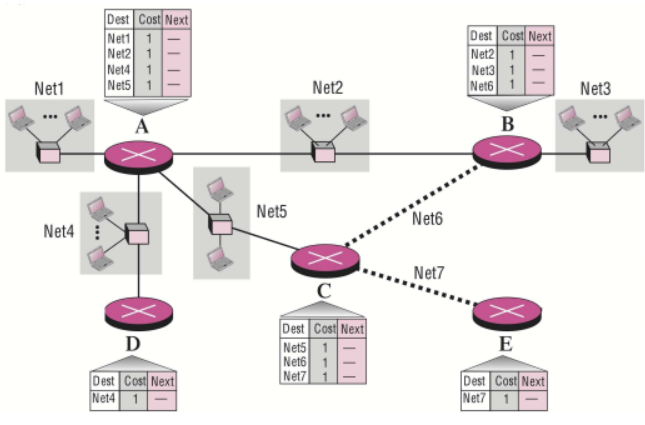
\includegraphics[width=0.8\textwidth]{assets/cap5/5.6.png}
\caption{Tabla de vectores de distancia inicial}
\label{fig:vectores-inicial}
\end{figure}

\subsection{Ejemplo de intercambio}

Inicialmente solo se conocen rutas directas. Tras el intercambio, cada router conoce la mejor ruta a todos los destinos.

\begin{figure}[H]
\centering
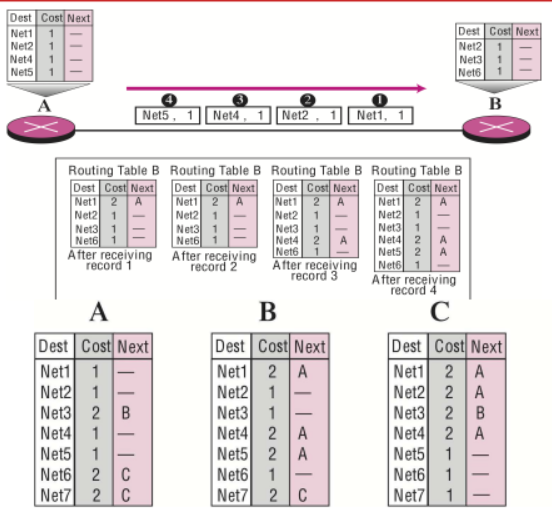
\includegraphics[width=0.8\textwidth]{assets/cap5/5.7.png}
\caption{Intercambio de vectores de distancia}
\label{fig:intercambio-vectores}
\end{figure}

\subsection{Problema: Cuenta a infinito}

Cuando un enlace cae o aumenta su coste, los cambios tardan en propagarse. Puede no converger debido a actualizaciones circulares que incrementan la metrica.

\begin{definicion}
La \textbf{cuenta a infinito (count-to-infinity)} es un problema de los protocolos por vectores de distancia en el que, tras un cambio negativo en la topologia, los routers incrementan ciclicamente sus metricas hasta alcanzar el limite establecido, provocando una convergencia muy lenta.
\end{definicion}

\subsection{Soluciones a la cuenta a infinito}

\begin{enumerate}
    \item \textbf{Limitar el infinito}: en RIP, 16 saltos = inalcanzable.
    \item \textbf{Horizonte dividido (split horizon)}: no se anuncia una ruta por la interfaz por la que se aprendio.
    \item \textbf{Horizonte dividido con respuesta envenenada (poisoned reverse)}: se anuncia con distancia infinita.
    \item \textbf{Actualizaciones forzadas (triggered updates)}: ante un cambio, se difunde inmediatamente.
\end{enumerate}

\begin{figure}[H]
\centering
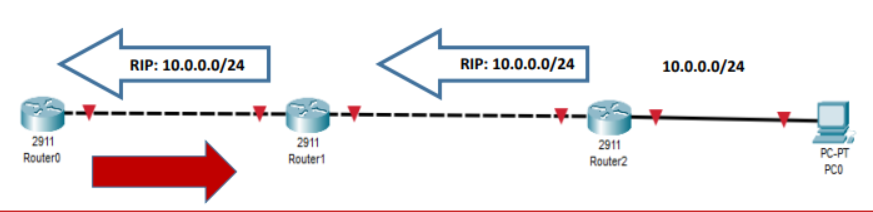
\includegraphics[width=0.8\textwidth]{assets/cap5/5.8.png}
\caption{Split horizon}
\label{fig:split-horizon}
\end{figure}

\begin{figure}[H]
\centering
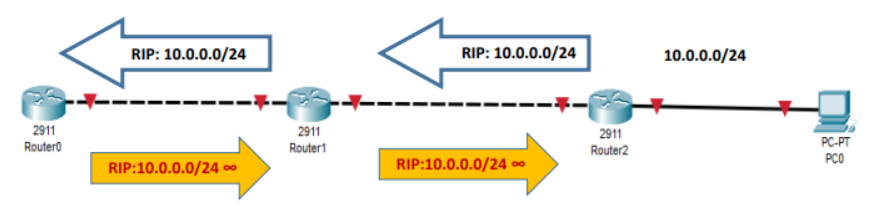
\includegraphics[width=0.8\textwidth]{assets/cap5/5.9.png}
\caption{Split horizon con poisoned reverse}
\label{fig:poisoned-reverse}
\end{figure}


\section{Encaminamiento en Internet}

\subsection{Sistemas Autonomos (AS)}

\begin{definicion}
Un \textbf{Sistema Autonomo (AS)} es un conjunto de redes y routers gestionados por una misma autoridad. Los \textbf{routers internos} usan protocolos IGP y solo conocen la organizacion de su AS. Los \textbf{routers frontera} (border routers) usan protocolos EGP y conocen el camino a otros AS, pero no su organizacion interna.
\end{definicion}

\begin{figure}[H]
\centering
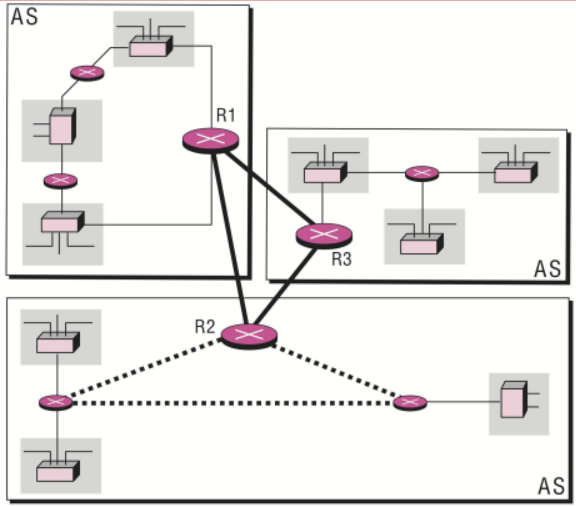
\includegraphics[width=0.8\textwidth]{assets/cap5/5.10.png}
\caption{Estructura de Internet con sistemas autonomos}
\label{fig:sistemas-autonomos}
\end{figure}

\subsection{Protocolos IGP (interior)}

\begin{itemize}
    \item \textbf{RIP} -- Routing Information Protocol
    \item \textbf{OSPF} -- Open Shortest Path First
    \item \textbf{IGRP} -- Internal Gateway Routing Protocol (Cisco)
\end{itemize}

\subsection{Protocolos EGP (exterior)}

\begin{itemize}
    \item \textbf{EGP} -- External Gateway Protocol
    \item \textbf{BGP} -- Border Gateway Protocol
\end{itemize}


\section{Practica 5: Encaminamiento en Internet con RIP}
\label{sec:practica5}

\subsection{Objetivos}

El objetivo de esta practica es profundizar en el concepto de encaminamiento en
redes de computadores, configurando routers con el protocolo de encaminamiento
\textbf{RIP} (Routing Information Protocol) en el simulador Cisco Packet Tracer.

\begin{enumerate}
    \item Comprender la diferencia entre encaminamiento estatico y dinamico.
    \item Configurar el protocolo RIP version 2 en multiples routers.
    \item Verificar que los routers intercambian informacion de rutas y convergen
    a la topologia de red.
    \item Comprobar la conectividad entre diferentes redes mediante traceroute y ping.
\end{enumerate}

\subsection{Material utilizado}

\begin{itemize}
    \item \textbf{Software}: Cisco Packet Tracer.
    \item \textbf{Hardware simulado}: 4 routers interconectados mediante enlaces seriales.
    \item \textbf{Redes involucradas}:
    \begin{itemize}
        \item 192.168.10.0/24 (LAN conectada a Router 0)
        \item 192.168.20.0/24 (LAN conectada a Router 3)
        \item 10.10.10.0/24 (enlace entre Router 0 y Router 2)
        \item 10.10.20.0/24 (enlace entre Router 1 y Router 2)
        \item 10.10.30.0/24 (enlace entre Router 0 y Router 1)
        \item 10.10.40.0/24 (enlace entre Router 2 y Router 3)
    \end{itemize}
\end{itemize}

\subsection{Desarrollo de la practica}

\subsubsection{Topologia de la red}

Se diseno una red con 4 routers interconectados mediante enlaces seriales,
formando una topologia mallada. Cada router tiene al menos una LAN conectada:

\begin{itemize}
    \item \textbf{Router 0}: conectado a la LAN 192.168.10.0/24 y a los enlaces
    10.10.10.0/24 (hacia Router 2) y 10.10.30.0/24 (hacia Router 1).
    \item \textbf{Router 1}: conectado al enlace 10.10.20.0/24 (hacia Router 2) y
    10.10.30.0/24 (hacia Router 0).
    \item \textbf{Router 2}: conectado a los enlaces 10.10.10.0/24 (hacia Router 0),
    10.10.20.0/24 (hacia Router 1) y 10.10.40.0/24 (hacia Router 3).
    \item \textbf{Router 3}: conectado a la LAN 192.168.20.0/24 y al enlace
    10.10.40.0/24 (hacia Router 2).
\end{itemize}

\begin{figure}[H]
\centering
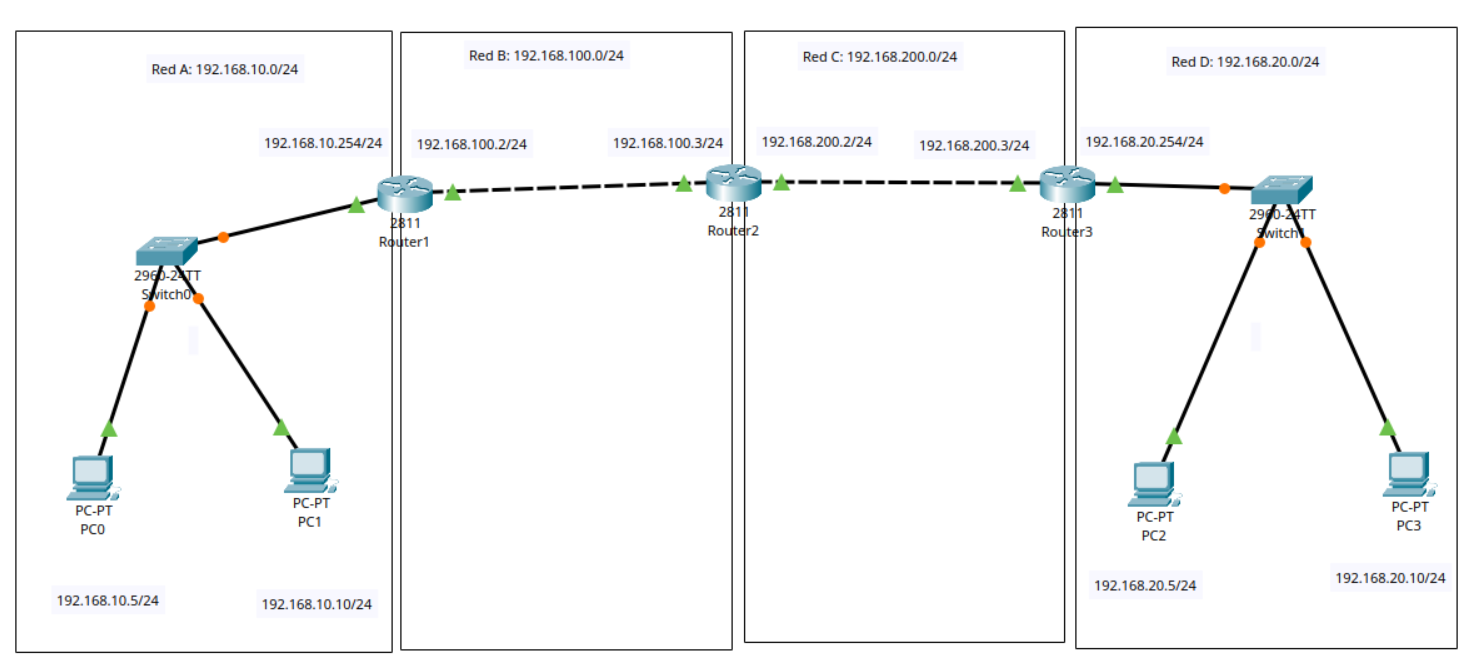
\includegraphics[width=0.8\textwidth]{assets/cap5/5.11.png}
\caption{Topologia de la red con 4 routers y encaminamiento RIP}
\label{fig:topologia-rip}
\end{figure}

\subsubsection{Configuracion de RIP en los routers}



\subsection{Relacion teoria-practica}

\begin{table}[htbp]
\centering
\small
\caption{Conexion entre conceptos teoricos y elementos de la Practica 5}
\begin{tabularx}{\textwidth}{@{}lX@{}}
\toprule
\textbf{Concepto teorico} & \textbf{Observacion/aplicacion en la practica} \\
\midrule
Encaminamiento estatico & Configuracion manual previa de rutas (alternativa mostrada en el enunciado) \\
Encaminamiento dinamico & RIP permite que los routers aprendan rutas automaticamente sin intervencion manual \\
Protocolo RIP (vector distancia) & Cada router intercambia periodicamente su tabla con los vecinos, usando saltos como metrica \\
Convergencia & Tras configurar RIP, los routers necesitan un tiempo para intercambiar tablas y alcanzar rutas estables \\
Tabla de encaminamiento & \texttt{show ip route} muestra rutas directamente conectadas (C) y aprendidas por RIP (R) \\
Distancia administrativa & 120 es la distancia administrativa de RIP; menor valor implica mayor confianza \\
Metrica de saltos & \texttt{[120/2]} indica 2 saltos hasta la red remota; RIP maximo 15 saltos \\
Next-hop & \texttt{via 10.10.10.2} indica la direccion IP del siguiente router al que reenviar el paquete \\
TTL (Time To Live) & El TTL decrece en cada salto; un valor de 253 indica 3 routers atravesados \\
Passive-interface & Evita enviar actualizaciones RIP por la interfaz LAN, reduciendo trafico innecesario \\
\bottomrule
\end{tabularx}
\end{table}


\section{Resumen de la Unidad 5}

\begin{itemize}
    \item El \textbf{encaminamiento} es la eleccion del camino optimo para un paquete; la \textbf{conmutacion} es el reenvio por ese camino.
    \item Los \textbf{grafos} modelan las redes: nodos son routers, enlaces son conexiones. Se representan mediante listas o matrices de adyacencia.
    \item Los \textbf{algoritmos de camino mas corto} como Dijkstra y Bellman-Ford permiten calcular rutas optimas. El \textbf{Minimum Spanning Tree} es util para difusion y evitacion de bucles.
    \item Las \textbf{tablas de encaminamiento} almacenan destino, mascara, siguiente salto y coste. El principio \textbf{next-hop} permite que cada router solo conozca el siguiente paso.
    \item Las \textbf{tecnicas de encaminamiento} incluyen: local (aleatorio, aislado, flooding), estatico (manual) y dinamico (vectores de distancia o estado de enlace).
    \item El \textbf{encaminamiento por vectores de distancia} usa Bellman-Ford e intercambio periodico de tablas. Sufre el problema de \textbf{cuenta a infinito}, resuelto con horizonte dividido, poisoned reverse y triggered updates.
    \item Los \textbf{protocolos de encaminamiento} se clasifican en: vector de distancia (RIP, Bellman-Ford) y estado de enlace (OSPF, Dijkstra).
    \item El \textbf{encaminamiento jerarquico} organiza Internet en Sistemas Autonomos (AS), usando protocolos IGP (RIP, OSPF) internamente y EGP (BGP) entre AS.
    \item \textbf{RIP} es un protocolo IGP por vectores de distancia con metrica de saltos, limite de 16, temporizadores periodicos (30s), de expiracion (180s) y de basura (120s).
    \item La \textbf{Practica 5} demuestra la configuracion de RIPv2 en una red de 4 routers, la convergencia de tablas, la verificacion con \texttt{show ip route}, \texttt{ping} y \texttt{traceroute}.
\end{itemize}
